
\chapter{Applied devices}


	\section{Arduino IDE}
	
		\hspace{15pt}We used Version 1.0.6 of the Arduino IDE to program the Arbotix-M microcontroller. The Arduino IDE is an open-source software which can be used to implement, compile and upload our codes to the microcontroller. The IDE can run on Linux and Mac OS as well as on Windows. Everyone can use the IDE to program any Arduino or Arduino based microcontroller like the Arbotix-M. The environment was created in Java and with other open-source and free software. Arduino has lots of advantages like: easy way to use, huge community who use Arduino, so they can help through online communication. \cite{arduino1} \cite{arduino2}
	
			\begin{figure}[ht]
				\centering
				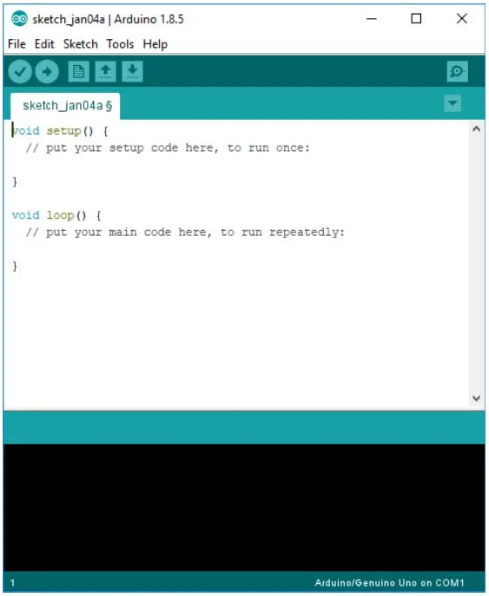
\includegraphics[scale=0.65]{./images/arduino_ide}
				\caption{Arduino IDE \cite{arduino_ide}}
			\end{figure}
			
			\newpage
		
	\section{Arbotix-m Robocontroller}
	
		\hspace{15pt}This is a versatile Arduino based robot controller method for systems which based in BIOLOID and DYNAMIXEL. Moreover this controller allows direct connection between the Dynamixel network and the board. ArbotiX-M Robocontroller has lots of advantages, as another Arduino compatible microcontroller, for example open source community of libraries and examples. The main difference between Arbotix and Arbotix M are the following: 
		
		\begin{itemize}
			\item In name of Arbotix M m stand for mini, cause it’s smaller than Arbotix.
			\item A smaller footprint(61mm X 61mm)
			\item 10 more general purpose I/O pins
			\item Barrel Jack for DC Power
			\item Separate Power Bus for 4 PWM Digital outputs for Hobby Servos
			\item No dedicated I2C header (I2C is still available on D16 = SCL D17=SDA)
			\item No DC Brushed Motor Controller
			\item Not compatible with the RX-Bridge
		\end{itemize}
		
		So the Arbotix-M has the following properties:
		
		\begin{itemize}
			\item 16MHz processor (ATMEG644p)
			\item 2 serial ports, these make easy to program using FTDI to USB connection.
			\item 3 TTL Dynamixel network interfacing ports (for direct motor connection)
			\item Analog and digital pins
		\end{itemize}

		Last but not least arbotixM robocontroller has a big disadvantage. Usually we said: Arbotixm is cheaper compare to the overall price of robots. Because of this, it’s not got the fastest processors or the best memory.
	
	\section{Pincher Robotic Arm}
	
		\hspace{15pt}The robot arm is a 5 degree-of-freedom robotic arm. This means the robot arm can can rotate along 5 different axes. \cite{arduino1}
		
		\begin{table}[ht]
			\begin{tabular}{|l|l|}
				\hline
				\multicolumn{2}{|l|}{\textbf{Pincher Robotic Arm Specification}} \\ \hline
				Weight                                & 550G                     \\ \hline
				Vertical Reach                        & 35CM                     \\ \hline
				Horizontal Reach                      & 31CM                     \\ \hline
			\end{tabular}
		\end{table}
		
		\subsection{Servo motor}
	
			\hspace{15pt}We have used Dynamixel AX-12A Robot Actuator servos in our project. The are powerful, durable and they have diagnostic functions too. They can monitor their voltage, and it is very important in protecting our battery from the damages of a critical undervoltage situation.

			These servos can measure their rotating angle, so they can be controlled very precisely. \cite{robot_servo}
			
			\begin{table}[ht]
				\begin{tabular}{|l|l|}
					\hline
					\multicolumn{2}{|l|}{\textbf{Servo motor specification}}                                                                              \\ \hline
					Weight               & 53.5g (AX-12/AX-12+), 54.6g (AX-12A)                                                                           \\ \hline
					Dimension            & 32mm * 50mm * 40mm                                                                                             \\ \hline
					Resolution           & 0.29°                                                                                                          \\ \hline
					Gear Reduction Ratio & 254 : 1                                                                                                        \\ \hline
					Stall Torque         & 1.5N.m (at 12.0V, 1.5A)                                                                                        \\ \hline
					No load speed        & 59rpm (at 12V)                                                                                                 \\ \hline
					Running Degree       & 0                                                                                                              \\ \hline
					Running Temperature  & -5°C $\sim$+70°C                                                                                                 \\ \hline
					Voltage              & 9 $\sim$12V (Recommended Voltage 11.1V)                                                                        \\ \hline
					Command Signal       & Digital Packet                                                                                                 \\ \hline
					Protocol Type        & \begin{tabular}[c]{@{}l@{}}Half duplex Asynchronous Serial Communication\\ (8bit,1stop,No Parity)\end{tabular} \\ \hline
					Link (Physical)      & TTL Level Multi Drop (daisy chain type Connector)                                                              \\ \hline
					ID                   & 254 (0-253)                                                                                                    \\ \hline
					Communication Speed  & 7343bps $\sim$1 Mbps                                                                                           \\ \hline
					Feedback						 & Position, Temperature, Load, Input Voltage, etc.																																\\ \hline
					Material						 & Engineering Plastic																																														\\ \hline
				\end{tabular}
			\end{table}

		\subsection{Pincher tool}
	
			\hspace{15pt}Our robot arm uses a so called pincher tool. Its maximum width is <> centimeters. It can produce a <> N holding force when closed. This tool is controlled by the fifth servo of the system, and it is made from industrial plastic too. \cite{robot_servo} \cite{pincher}
		
				\begin{figure}[ht]
					\centering
					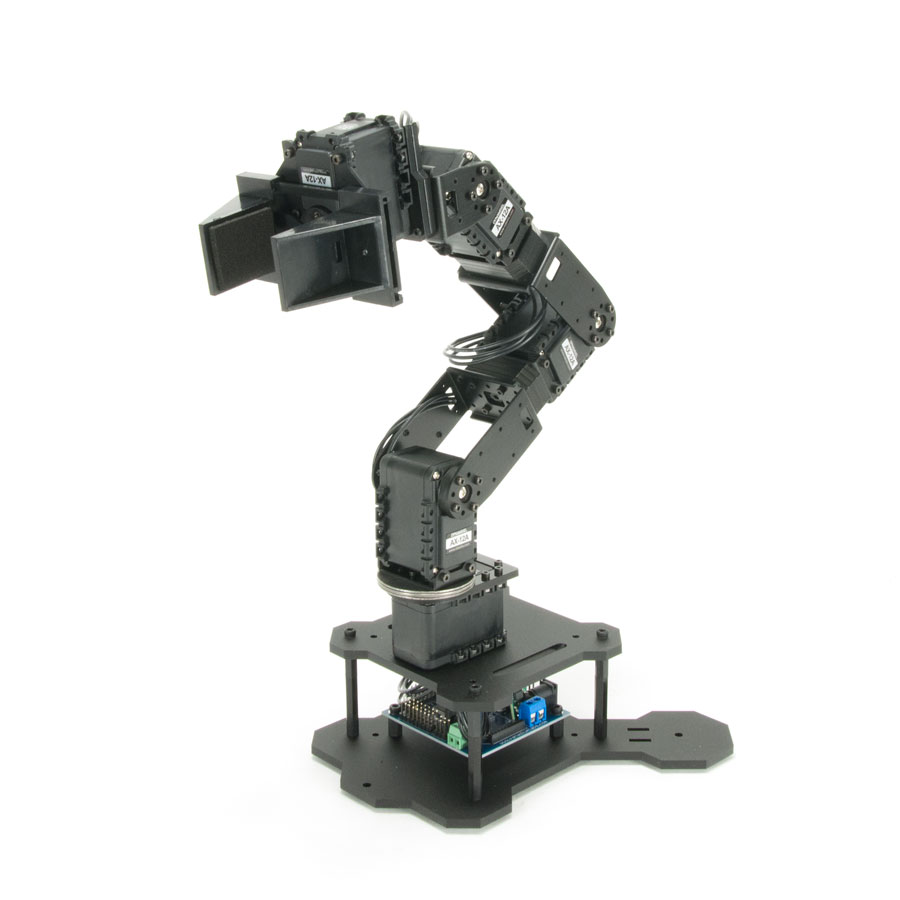
\includegraphics[scale=0.33]{./images/pincher}
					\caption{Pincher \cite{pincher}}
				\end{figure}
	
	\section{Programming language}
		\hspace{15pt}Arduino doesn't run either C or C++. It runs machine code that compiled from C, C++ or any other language. The Arduino IDE accepts C and C++ as it is. Most of the libraries are written in C++, but it is very different from most C++ varieties. The Arduino C++ language has a lot of abstraction built in.
		
		
		Most of the embedded systems in the microcontroller world are using C++ language. Arduino code's core functions are simply a set of the C++ classes and libraries. Arduino language simplifies a lot of things, but we can still write our functions as we want and where we need more specialization. 